% Included from both -slides and -handout versions.

\mode<presentation>
{
  \usetheme{default}
  \useoutertheme{infolines}
}

\usepackage[english]{babel}
\usepackage[latin1]{inputenc}
\usepackage{graphicx}
\usepackage{times}
\usepackage[T1]{fontenc}
\usepackage{fancyvrb}
\usepackage{listings}
\begin{document}
\lstset{language=C, escapeinside={(*@}{@*)}, numbers=left,
  basicstyle=\tiny, showspaces=false, showtabs=false}

\def\Tiny{\fontsize{4pt}{4pt} \selectfont}

\title{L41 - Lecture 6: The Network Stack (2)}
%\institute{University of Cambridge}
%\author{George V. Neville-Neil}
\author{Dr Robert N. M. Watson}
\date{22 January 2016}

\begin{frame}
  \titlepage
\end{frame}

\section{Introduction}

\begin{frame}
  \frametitle{Reminder: Last time}

  \begin{enumerate}
    \item Networking and the sockets API
    \item Network-stack design principles
    \item Memory flow in hardware and software
    \item Network-stack construction and work flows
    \item A couple of pieces of recent network-stack research
  \end{enumerate}
\end{frame}

% \section{Socket buffers}

% The socket data structure

% What is a socket buffer?

% Application/socket flow control

\section{TCP protocol}

\begin{frame}[fragile]
  \frametitle{The Transmission Control Protocol (TCP)}

  \begin{columns}[T]
    \column{0.45\textwidth}

  \begin{Tiny}
    \begin{verbatim}
September 1981                             Transmission Control Protocol
                                                Functional Specification

                              +---------+ ---------\      active OPEN  
                              |  CLOSED |            \    -----------  
                              +---------+<---------\   \   create TCB  
                                |     ^              \   \  snd SYN    
                   passive OPEN |     |   CLOSE        \   \           
                   ------------ |     | ----------       \   \         
                    create TCB  |     | delete TCB         \   \       
                                V     |                      \   \     
                              +---------+            CLOSE    |    \   
                              |  LISTEN |          ---------- |     |  
                              +---------+          delete TCB |     |  
                   rcv SYN      |     |     SEND              |     |  
                  -----------   |     |    -------            |     V  
 +---------+      snd SYN,ACK  /       \   snd SYN          +---------+
 |         |<-----------------           ------------------>|         |
 |   SYN   |                    rcv SYN                     |   SYN   |
 |   RCVD  |<-----------------------------------------------|   SENT  |
 |         |                    snd ACK                     |         |
 |         |------------------           -------------------|         |
 +---------+   rcv ACK of SYN  \       /  rcv SYN,ACK       +---------+
   |           --------------   |     |   -----------                  
   |                  x         |     |     snd ACK                    
   |                            V     V                                
   |  CLOSE                   +---------+                              
   | -------                  |  ESTAB  |                              
   | snd FIN                  +---------+                              
   |                   CLOSE    |     |    rcv FIN                     
   V                  -------   |     |    -------                     
 +---------+          snd FIN  /       \   snd ACK          +---------+
 |  FIN    |<-----------------           ------------------>|  CLOSE  |
 | WAIT-1  |------------------                              |   WAIT  |
 +---------+          rcv FIN  \                            +---------+
   | rcv ACK of FIN   -------   |                            CLOSE  |  
   | --------------   snd ACK   |                           ------- |  
   V        x                   V                           snd FIN V  
 +---------+                  +---------+                   +---------+
 |FINWAIT-2|                  | CLOSING |                   | LAST-ACK|
 +---------+                  +---------+                   +---------+
   |                rcv ACK of FIN |                 rcv ACK of FIN |  
   |  rcv FIN       -------------- |    Timeout=2MSL -------------- |  
   |  -------              x       V    ------------        x       V  
    \ snd ACK                 +---------+delete TCB         +---------+
     ------------------------>|TIME WAIT|------------------>| CLOSED  |
                              +---------+                   +---------+

                      TCP Connection State Diagram
                               Figure 6.
\end{verbatim}
  \end{Tiny}

    \column{0.45\textwidth}
    \bigskip
    \begin{itemize}
      \item V. Cerf, K. Dalal, and C. Sunshine, \textit{Transmission Control
	Protocol (version 1)}, INWG General Note \#72, December 1974.
      \item In practice: Jon Postel, Ed, \textit{Transmission Control
	Protocol: Protocol Specification}, RFC 793, September, 1981.
    \end{itemize}
  \end{columns}

\end{frame}

% Rules of the game:
% - two endpoints can only communicate by packets
% - minimum RTT to see responses
% - network is allowed to delay, (reorder), drop, corrupt packets
% - no cheating: can't inspect remote state, only state sent on wire
% - there are other players on the network -- congestion, etc
% - middle nodes don't help (although, with ECN, they do a little)

% TCP header

% TCP handshake

\begin{frame}
  \frametitle{TCP goals and properties}

  \begin{columns}[T]
    \column{0.38\textwidth}
      \smallskip
      \begin{center}
	\includegraphics[width=1.15\textwidth]{../../figures/tcp-timeline.pdf}
      \end{center}

    \column{0.52\textwidth}
      \begin{itemize}
	\item Reliable, ordered, byte-stream transport protocol over IP
	%\item Connections identified by unique IP-port 4-tuple
	\item Three-way handshake: SYN~/ SYN-ACK~/ ACK (mostly!)
        \item Flow control via advertised window size in ACKs
	\item Congestion control via packet loss and ECN (`fairness')

	\pause

	\item Network may delay, (reorder), drop, corrupt packets
	\item Sequence numbers ACK'd; data retransmitted on loss
	\item Round-Trip Time (RTT) measured to time out loss

	%\pause

	%\item Complex teardown permits `half-close' and port reuse
      \end{itemize}

  \end{columns}
\end{frame}

\begin{frame}
  \frametitle{TCP congestion control and avoidance}

  \begin{columns}[T]
    \column{0.35\textwidth}
      \begin{center}
	\includegraphics[width=1.2\textwidth]{../../figures/vj-congestion-slow-start.pdf}
      \end{center}

    \column{0.55\textwidth}

      \begin{itemize}
	\item 1986 Internet CC collapse
	\begin{itemize}
	  \item 32Kbps -> 40bps
	\end{itemize}

	\pause

	\item Van Jacobson, SIGCOMM 1988
	\begin{itemize}
	  \item Don't send more data than the network can handle!
	  \item \textit{Conservation of packets} via \textit{ACK clocking}
	  \item \textit{Exponential retransmit timer}, \textit{slow start},
	    \textit{aggressive receiver ACK}, and \textit{dynamic window
	    sizing on congestion}
        \end{itemize}

	\pause

        \item ECN (RFC 3168), ABC (RFC 3465), Compound (Tan, et al, INFOCOM
	  2006), Cubic (Rhee and Xu, ACM OSR 2008)
      \end{itemize}
  \end{columns}
\end{frame}

\begin{frame}
  \frametitle{TCP time/sequence graphs}

  \begin{columns}[T]
    \column{0.4\textwidth}
      \bigskip
      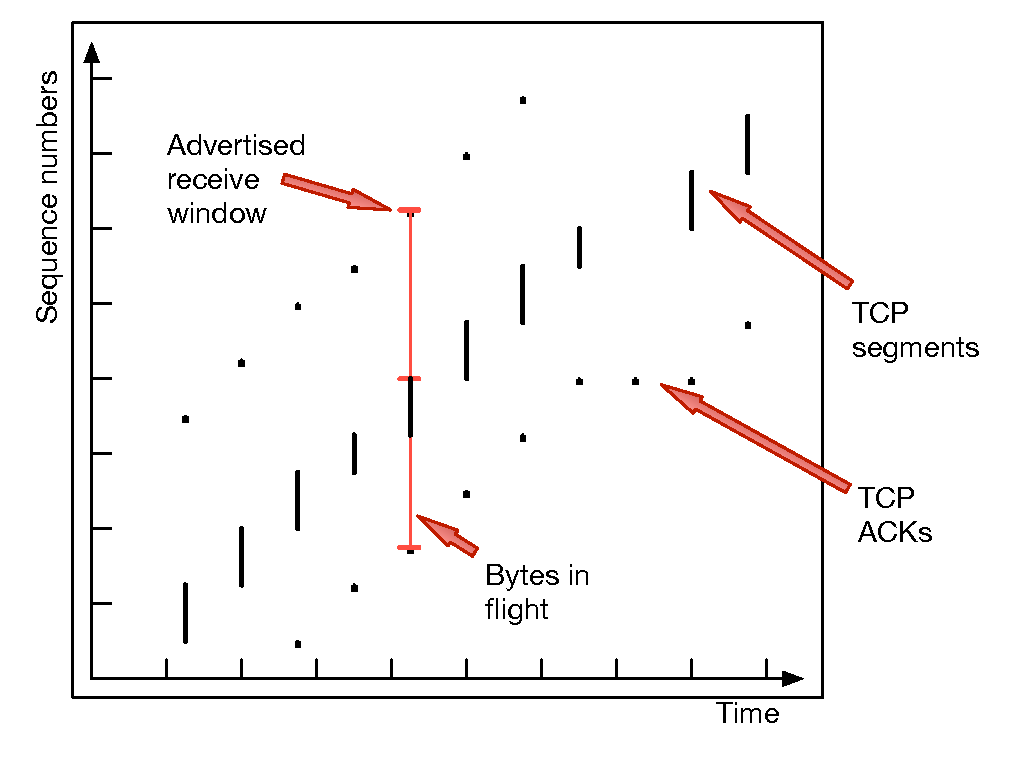
\includegraphics[width=1.25\textwidth]{../../figures/tcp-time-sequence.pdf}

    \column{0.5\textwidth}
    \begin{itemize}
      \item Extracted from bi-directional TCP packet traces
      \begin{itemize}
	\item Sequence numbers in data segments, advertised window,
	  acknowledgments
	\item X: time
	\item Y: sequence number
      \end{itemize}
      \item Visualise receive windows, congestion behaviour, RTT, ...
      \item We can also extract this data using DTrace
    \end{itemize}
  \end{columns}
\end{frame}

\section{TCP implementation}

\begin{frame}
  \frametitle{BSD/FreeBSD TCP implementation evolution}

  \begin{small}
  1983 - 4.2 BSD: BSD sockets, TCP/IP implementation \\
  1986 - 4.3 BSD: VJ/Karels congestion control \\

  \pause
  \medskip

  1999 - FreeBSD 3.1: \texttt{sendfile(2)} \\
  2000 - FreeBSD 4.2: TCP accept filters \\
  2001 - FreeBSD 4.4: TCP ISN randomisation \\
  2002 - FreeBSD 4.5: TCP SYN cache/cookies \\

  \pause
  \medskip

  2003 - FreeBSD 5.0--5.1: IPv6, TCP TIMEWAIT state reduction \\
  2004 - FreeBSD 5.2--5.3: TCP host cache, SACK, fine-grained locking  \\

  \pause
  \medskip

  2008 - FreeBSD 6.3: TCP LRO, TSO \\
  2008 - FreeBSD 7.0: T/TCP removed, socket-buffer autosizing \\
  2009 - FreeBSD 7.1: read-write locking, full TCP offload \\
  2009 - FreeBSD 8.0: TCP ECN \\
  2012 - FreeBSD 9.0: pluggable congestion control, connection groups
  \end{small}

  \begin{itemize}
    \item Which changes have protocol-visible effects vs. only code?
  \end{itemize}
\end{frame}

\begin{frame}
  \frametitle{Lect. 5: Local send/receive paths in the network stack}
  \begin{center}
    \includegraphics[scale=0.4]{../../figures/network-in-out.pdf}
  \end{center}
\end{frame}

\begin{frame}
  \frametitle{Data structures - sockets, control blocks}

  \begin{center}
    \includegraphics[width=\textwidth]{../../figures/tcp-structures.pdf}
  \end{center}
\end{frame}

\begin{frame}
  \frametitle{Denial of Service (DoS) - state minimisation}

  \begin{center}
    \includegraphics[width=.55\textwidth]{../../figures/tcp-syn-flood.pdf}
  \end{center}

  \begin{itemize}
    \item Yahoo!, Amazon, CNN taken out by SYN floods in February 2000
    \item D. Borman: TCP SYN cache - minimise state for new connection
    \item D. Bernstein: SYN cookies - eliminate state entirely -- at a cost
    \item J. Lemon: TCP TIMEWAIT reduction - minimise state during close
    \item J. Lemon: TCP TIMEWAIT recycle - release state early under load
  \end{itemize}
\end{frame}

%\begin{frame}
%  \frametitle{TCP reassembly}
%
%
%\end{frame}
%
%\begin{frame}
%  \frametitle{TCP timers}
%
%
%\end{frame}

\begin{frame}
  \frametitle{TCP-connection lookup tables}

  \begin{center}
    \includegraphics[width=0.65\textwidth]{../../figures/tcp-hash-table.pdf}
  \end{center}

  \begin{itemize}
    \item Global list of connections for monitoring (e.g., \texttt{netstat})
    \item Connections are installed in a global hash table for lookup
    \item Separate (similar) hash table for port-number allocations
    \item Tables protected by global read-write lock as reads dominant
    \begin{itemize}
      \item New packets more frequent than new connections
    \end{itemize}
  \end{itemize}
\end{frame}

%
% XXX: Next year, talk about sendfile() and I/O lite to consider the steady
% state?
%

\begin{frame}
  \frametitle{Lect. 5 - Work dispatch: input path}

  \begin{center}
    \includegraphics[width=0.9\textwidth]{../../figures/network-dispatch-input.pdf}
  \end{center}

  \begin{small}
  \begin{itemize}
    \item Deferred dispatch - \textit{ithread} -> \textit{netisr thread} ->
      \textit{user thread}
    \item Now: direct dispatch - \textit{ithread} -> \textit{user thread}
    \begin{itemize}
      \item Pros: reduced latency, better cache locality, drop overload early
      \item Cons: reduced parallelism and work placement opportunities
    \end{itemize}
  \end{itemize}
  \end{small}
\end{frame}

\begin{frame}
  \frametitle{An Evaluation of Network Stack Parallelization Strategies in
    Modern Operating Systems}

  Paul Willmann, Scott Rixner, and Alan L. Cox, USENIX ATC, 2006.

  \smallskip

  \begin{columns}[T]
    \column{0.27\textwidth}
      \begin{center}
	\includegraphics[width=1.1\textwidth]{../../figures/tcp-mp-strategies.pdf}
      \end{center}

    \column{0.63\textwidth}

      \begin{itemize}
	\item Network bandwidth growth > \\ CPU frequency growth
	\item Locking overhead (space, contention) substantial -- getting
	  `speedup' is hard
	\item Evaluate different strategies for TCP processing parallelisation
	\item Message-based Parallelism
	\item Connection-based Parallelism (threads)
	\item Connection-based Parallelism (locks)
	\item Coalescing locks for connections by hashing 4-tuples has
	  substantial benefit in overhead and parallelism
      \end{itemize}
  \end{columns}
\end{frame}

\begin{frame}
  \frametitle{FreeBSD connection groups, RSS}

  \begin{center}
    \includegraphics[width=0.6\textwidth]{../../figures/tcp-hash-table-groups.pdf}
  \end{center}

  \begin{itemize}
    \item Connection groups blend MsgP and ConnP-L models
      \begin{itemize}
	\item PCBs assigned to group based on 4-tuple hash
	\item Lookup requires group lock, not global lock
	\item Global lock retained for 4-tuple reservation (e.g., setup,
	  teardown)
	%\item Juggling needed for SYN/FIN/RST due to lock upgrades
      \end{itemize}
    \item Problem: have to look at TCP headers (cache lines) to place work!

    \pause

    \item Microsoft: NIC Receive-Side Scaling (RSS)
      \begin{itemize}
	\item Multi-queue NICs deliver packets to queue using hash
	\item Align connection groups with RSS buckets / interrupt routing
      \end{itemize}
  \end{itemize}
\end{frame}

\begin{frame}
  \frametitle{Performance: dispatch model and locking}

  \begin{columns}[T]
    \column{0.6\textwidth}
      \includegraphics[width=1.1\textwidth]{../../figures/2010-dispatch-variations.pdf}

    \column{0.3\textwidth}
      \begin{itemize}
	\item 2010-vintage 4-core x86 multicore
	\item TCP LRO disabled
	\item Single queue: \\ 1 ithread
	\item Single queue: \\ 8 worker threads \\ (1 per core)
	\item Multi queue: \\ 8 queues, \\ 8 ithreads
      \end{itemize}
  \end{columns}
\end{frame}

\begin{frame}
  \frametitle{From architectural to micro-architectural optimisation}

  \begin{itemize}
    \item Counting instructions -> counting cache misses
    \item Lock contention -> cache-line contention
    \item Locking -> identifying parallelism opportunities
    \item Work ordering, classification, and distribution
    \item NIC offload of further protocol layers, crypto
    \item Vertically integrate distribution and affinity
    \item DMA/cache interactions
  \end{itemize}
\end{frame}

\section{Conclusion}

\begin{frame}
  \frametitle{Labs 4 + 5: TCP}

  \begin{itemize}
    \item Build from abstract to more concrete understanding of TCP
    \item Use tools such as \texttt{tcpdump} and \texttt{DUMMYNET}
    \item Explore effects of latency on TCP performance
  \end{itemize}

  \begin{description}
    \item[Lab 4 - TCP state machine and latency] ~ \\
      \begin{itemize}
	\item Measure the TCP state machine in practice
	\item Explore TCP latency vs. bandwidth (DUMMYNET)
	\item At what transfer size are different latencies masked?
      \end{itemize}

    \item[Lab 5 - TCP congestion control] ~ \\
      \begin{itemize}
        \item Draw time--sequence-number diagrams
	\item Annotate diagrams with scheduler events
	\item Annotate diagrams with timer events
	\item Effects of latency on slow-start rampup
      \end{itemize}
  \end{description}
\end{frame}

\end{document}
